% Drawing 154/01-2 -- folder 154, batch 01, archive page 2 (PDF page 3).
% Transcription: figure : un disque dessiné en rouge, traversé par un arrangement de pseudo-droites, avec deux points noirs aux extrémités d'un diamètre horizontal et, en pointillé jaune, l'arc supérieur entre eux ; un trait séparateur au crayon descend entre les deux colonnes
% Kind: pseudoline arrangement in a disk. Method 2 (schematic redraw from the facsimile). Status: partial.
% Notes: A disk drawn in red, crossed by a red pseudoline arrangement, two black points at the ends of a horizontal diameter, and the upper arc between them dotted in yellow (drawn just inside the circle); the pencil separator running down between the columns. The red strands are redrawn schematically (about eight; their crossings are not all recoverable). Still differs from the facsimile: The red strands are redrawn schematically (about eight; their crossings are not all recoverable).
% Coordinates: 1 unit = 1 mm = 1/100 of the crop width (bbox in page fractions: [0.601, 0.329, 0.871, 0.52]).
% Redrawn by Claude (claude-opus-5-5), issue #73, 2026-11-07; not checked by a human; not compiled (no TeX in the session).
% Revised by Claude (claude-opus-5-5) 2026-11-09 (issue #128) after Michel's check: vertices snapped to exact intersections (drawn points on their lines, meeting ends on the stroke they meet, near-concurrent lines through one computed point, curve ends on their rim); labels at \small as in folder 80 batch 3. Status: partial.
% Rights: reproduces part of the work -- behind RENDER_TRANSCRIPTS, never published by itself.
\documentclass[tikz,border=3pt]{standalone}
\usepackage{amsmath,amssymb}
\usetikzlibrary{patterns,arrows.meta}
\tikzset{Or/.style={orange!90!black}, Ye/.style={yellow!80!orange}, Lg/.style={green!60!black!70}, Dg/.style={green!45!black}, Br/.style={brown!80!black}, Rd/.style={red!85!black}, Bl/.style={blue!70!black}, Gy/.style={black!40}, pencil/.style={black!45}, struck/.style={black!35}, mark/.style={circle,draw,inner sep=1.3pt}, pt/.style={circle,fill,inner sep=0.9pt}, opt/.style={circle,draw,fill=white,inner sep=1.1pt}}
\begin{document}
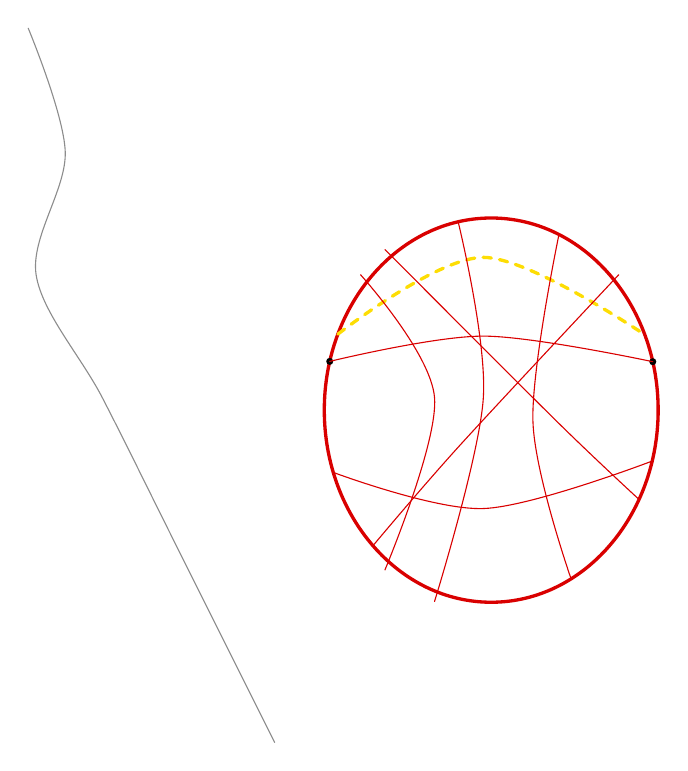
\begin{tikzpicture}[x=1mm,y=1mm,line cap=round,line join=round,font=\scriptsize]
\draw[Rd,very thick] (66.6,-51.6) ellipse[x radius=21.2, y radius=24.4];
\node[pt] at (46.09,-45.41) {};
\node[pt] at (87.12,-45.45) {};
\draw[Ye,dashed,very thick] plot[smooth, tension=0.55] coordinates {(47.13,-41.95) (65.6,-32.2) (86.1,-42.02)};
\draw[Rd] plot[smooth, tension=0.55] coordinates {(46.09,-45.41) (65.6,-42.2) (87.12,-45.45)};
\draw[Rd] plot[smooth, tension=0.55] coordinates {(50,-34.4) (59.4,-50) (53.1,-71.9)};
\draw[Rd] plot[smooth, tension=0.55] coordinates {(62.4,-27.68) (65.6,-50) (59.4,-75.9)};
\draw[Rd] plot[smooth, tension=0.55] coordinates {(75.2,-29.3) (71.9,-53.1) (76.74,-73.03)};
\draw[Rd] plot[smooth, tension=0.55] coordinates {(53.1,-31.2) (75,-53.1) (85.37,-62.94)};
\draw[Rd] plot[smooth, tension=0.55] coordinates {(82.8,-34.4) (62.5,-56.2) (51.58,-68.82)};
\draw[Rd] plot[smooth, tension=0.55] coordinates {(46.54,-59.51) (65.6,-64.1) (87.04,-58.07)};
\draw[pencil] plot[smooth, tension=0.55] coordinates {(7.8,-3.1) (12.5,-18.8) (8.8,-34.4) (17.2,-50) (26.6,-68.8) (39.1,-93.8)};
\end{tikzpicture}
\end{document}
